\chapter{Orientation Estimation Using MARG Sensors}
\label{ch:orientation_estimation}

This chapter covers the working principals of MARG sensors, as well as the fundamentals of orientation estimation, that are necessary for the implementation of the aforementioned system. Subsequently, a mathematical construct used to express orientation -- Euler angles -- is explained. Towards the end of the chapter, different approaches to compute orientation estimates from magnetic and inertial data including their pros and cons are described. Finally, sensor fusion as a means to mitigate the drawbacks of each approach is introduced.

\section{MARG Sensors}

MARG sensors is a collective term for magnetic, angular rate, and gravitational sensors, which encompasses inertial sensors, as well as magnetic field sensors, also referred to as magnetometers. Inertial sensors itself generally fall into two categories: instruments sensing linear inertial displacement, i.\,e. accelerometers, and rotational inertial rate sensors, that is gyroscopes. They are applied in various contexts to quantify vibration, motion, and shock \cite{bhattacharyya_inertial_sensors_applications_13}. Particularly, the development of \gls{MEMS} opened up many medical applications as stated in Section \ref{sec:MARG_sensors_medical}. MEMS sensors have low manufacturing costs, small physical size, and low power consumption \cite{bhattacharyya_inertial_sensors_applications_13}. This section compiles the functional principles of different MARG sensors and introduces \glspl{IMU} as a combination of those.

\subsection{Accelerometers}\label{sec:accelerometers}

Accelerometers measure the acceleration of an object relative to an inertial frame. Since acceleration cannot be sensed directly, the force exerted on a reference mass is measured. The resultant acceleration is computed according to Newton's second law $\mathbf{f} = m \cdot \mathbf{a}$, where $\mathbf{f} \in \mathbb{R}^3$ denotes the force vector, $m$ the mass, and $\mathbf{a} \in \mathbb{R}^3$ the acceleration vector. Usually, a single axis accelerometer consists of a small proof mass connected via a spring to the case of the instrument. The proof mass is displaced  by $\Delta x$ with respect to the case, when the instrument experiences a certain acceleration along its sensitive axis. Disregarding drag force, according to Hooke's law $f = -k \cdot \Delta x$, the displacement is directly proportional to the force exerted by the mass and thus to the acceleration. Therefore, by measuring the displacement of the proof mass the acceleration can be obtained. Figure \ref{fig:accelerometer} shows the displacement $\Delta x$ of the mass with respect to the case of the instrument for three different conditions: (a) at rest or in uniform motion, (b) accelerating, and (c) at rest, being exposed to the gravity $ \mathbf{g}$. According to how the mass displacement is sensed, accelerometers can be classified as resistive, capacitive, and piezoelectric. Besides, there are surface acoustic wave, fibre optic, vibrating beam and solid-state \gls{MEMS} accelerometers. To obtain a three-dimensional accelerometer, three single-axis accelerometers are mounted together. Nowadays, most accelerometers are manufactured using MEMS technology, which was developed for the military and aerospace markets in the 1970s \cite{bhattacharyya_inertial_sensors_applications_13}. 

\begin{figure}
\centering
\begin{tikzpicture}[scale=0.95, auto, thick, node distance=3cm,>=latex']
    \pgftext{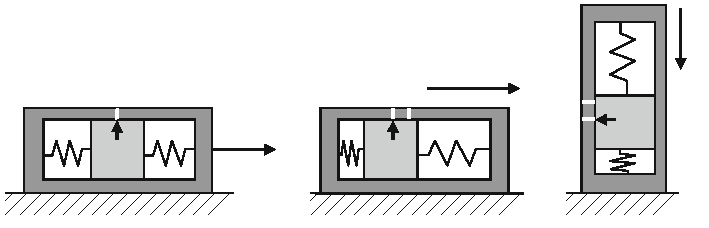
\includegraphics[width=13.5cm]{Figures/accelerometer}} at (0pt,0pt);
    \node [] (a) at (-6.7, -1.1) {(a)};
    \node [] (b) at (-1.1, -1.1) {(b)};
    \node [] (c) at (3.9, -1.1) {(c)};
    \node [] (c) at (-4.525, 0.44) {$0$};
    \node [] (c) at (1.03, 0.44) {$0$};
    \node [] (c) at (4, 0.26) {$0$};
    \node [] (c) at (0.58, 0.44) {$\Delta x$};
    \node [] (c) at (3.82, -0.08) {$\Delta x$};
    \node [] (c) at (6.5, 1.5) {$\mathbf{g}$};
    \node [] (c) at (-4.525, -0.75) {\scriptsize Proof};
    \node [] (c) at (-4.525, -1.05) {\scriptsize mass};
    \node [] (c) at (-2, -0.05) {\scriptsize Sensitive};
    \node [] (c) at (-2, -0.45) {\scriptsize axis};
    \node [] (c) at (2.2, 0.82) {$\mathbf{a}$};
\end{tikzpicture}
\caption{A mass-and-spring accelerometer under different conditions: (a) at rest or in uniform motion, (b) accelerating, and (c) at rest, being exposed to the gravity $\mathbf{g}$, from \cite{bhattacharyya_inertial_sensors_applications_13}.}
	\label{fig:accelerometer}
\end{figure}


\subsection{Gyroscopes}

Gyroscopes are used for measuring and maintaining angular orientation. In essence, based on two different physical principles, namely the Sagnac and Coriolis effect, gyroscopes sense angular velocity, which is why they are also referred to as angular velocity sensors or angular rate sensors. By integrating the angular velocity the rotation angle can be obtained. Here we will only elaborate on the working principle of vibrating gyroscopes, since they are utilised in the GaitWatch system. \citeauthor{armenise2010advances} give a comprehensive overview of current gyroscope technologies in \cite{armenise2010advances}.

Coriolis vibratory gyroscopes, or vibrating gyros for short, sense angular velocity based on the effect of Coriolis force on a vibrating mass. The Coriolis force is a fictitious force experienced by a mass $m$ moving in a rotating reference frame. It can be calculated as: $\mathbf{f}_C = -2m(\bm{\omega} \times \mathbf{v})$, where $\mathbf{v}$ is the mass velocity in the rotating reference frame and $\bm{\omega}$ is the angular velocity of the reference frame. As seen in this equation the Coriolis force is only present when the mass varies its distance with respect to the spin axis. Otherwise, if $\bm{\omega}$ and $\mathbf{v}$ are parallel, the cross product becomes zero. The two degree-of-freedom spring-mass-damper system shown in Figure \ref{fig:gyroscope} serves as a simple model of a vibrating angular rate sensor. The mass $m$ can move along the $x$ and $y$-axis, respectively. The angular velocity around the $z$-axis is denoted with $\omega$. The drive or primary oscillating mode, that is, the oscillation along $x$, is excited by the force $F_x$ directed along the $x$-axis. The oscillation along $y$, called sense or secondary oscillating mode, is due to system rotation around the $z$-axis. $D_x$ and $D_y$ are the damping coefficients and $k_x$ and $k_y$ are the spring constants along the $x$ and $y$-axis, respectively. Typically, the primary oscillating mode is excited by a sinusoidal force with an angular frequency close to the resonance frequency, so that $\Omega_x \cong \sqrt{k_x/m}$. Its amplitude is kept constant at $a_x$. As shown in \cite{armenise2010advances}, the amplitude of the sense mode is then given by

\begin{equation}
  a_y = -\frac{2 a_x \Omega_x \omega}{\sqrt{(\Omega^2_x - \Omega^2_y)^2 + \Omega^2_x \Omega^2_y / Q^2_y}}\,,
\end{equation}

\noindent
where $\Omega_y=\sqrt{k_y/m}$ is the resonance frequency of the secondary resonator and $Q_y = \sqrt{m k_y}/D_y$ its quality factor. The amplitude $a_y$ is directly proportional to the angular rate of the two degree-of-freedom spring-mass-damper system. Thus, $\omega$ can be estimated by measuring the amplitude of the oscillation along the $y$-axis.

Usually, vibrating gyroscopes are manufactured using MEMS technology. MEMS gyros are of low to medium accuracy \cite{bhattacharyya_inertial_sensors_applications_13}, but due to their size they are ideally suited for medical applications.

\begin{figure}
\centering
\begin{tikzpicture}[auto, thick,>=latex', cross/.style={path picture={ 
  \draw[black]
(path picture bounding box.south east) -- (path picture bounding box.north west) (path picture bounding box.south west) -- (path picture bounding box.north east); }}]

\tikzstyle{spring}=[thick,decorate,decoration={zigzag,pre length=0.3cm,post length=0.3cm,segment length=6}]
\tikzstyle{damper}=[thick,decoration={markings,  
  mark connection node=dmp,
  mark=at position 0.5 with 
  {
    \node (dmp) [thick,inner sep=0pt,transform shape,rotate=-90,minimum width=8pt,minimum height=7pt,draw=none] {};
    \draw [thick] ($(dmp.north east)+(4pt,0)$) -- (dmp.south east) -- (dmp.south west) -- ($(dmp.north west)+(4pt,0)$);
    \draw [thick] ($(dmp.north)+(0,-4pt)$) -- ($(dmp.north)+(0,4pt)$);
  }}, decorate]
\tikzstyle{ground}=[fill,pattern=north east lines,draw=none,minimum width=0.75cm,minimum height=0.3cm]


\node (M) [draw, minimum width=3cm, minimum height=3cm] {};

\node (ground) [ground,anchor=north,yshift=-1.5cm,minimum width=3.5cm] at (M.south) {};
\draw (ground.north east) -- (ground.north west);

\node (wall) [ground, rotate=-90, minimum width=3.5cm,yshift=-3cm] {};
\draw (wall.north east) -- (wall.north west);

\draw [spring] (wall.170) -- node [label={[label distance=-0.2cm]above:$k_x$}] {}($(M.north west)!(wall.170)!(M.south west)$);
\draw [damper] (wall.10) -- node [label={[label distance=-0.1cm]above:$D_x$}] {}($(M.north west)!(wall.10)!(M.south west)$);

\draw [spring] (ground.170) -- node [label={[label distance=0.09cm]right:$k_y$}] {}($(M.south east)!(ground.170)!(M.south west)$);
\draw [damper] (ground.10) -- node [label={[label distance=0.08cm]right:$D_y$}] {}($(M.south east)!(ground.10)!(M.south west)$);      

    \node[coordinate] (X) at (5,-1) {};
    \node[coordinate] (Y) at (3,1) {};
    \node[coordinate] (O) at (3, -1) {};
    
    \draw[->] (O) -- node[name=x] {$x$}(X);
    \draw[->] (O) -- node[name=y] {$y$}(Y);
    \node [draw,circle, fill=white,cross,minimum width=0.15 cm, label={[anchor=south west]below:$z$}](z) at (3, -1){};
    
    \draw[-stealth] (0.15,1) arc (80:390:1);
    
    \node at (0.6, 0.8) (angle1) {$\omega$};
    \node at (-1.05, 1.1) (angle1) {$m$};
    
    \draw [-stealth, align=center] (-0.5,2) -- node[name=Fx] {$F_x$} (0.5,2);

    
\end{tikzpicture}
\caption{A simple model of a Coriolis vibratory gyroscope: A two degree-of-freedom spring-mass-damper system in a rotating reference frame, from \cite{armenise2010advances}.} \label{fig:gyroscope}
\end{figure} 
 

\subsection{Magnetometers}

Magnetometers measure the strength and the direction of the magnetic field at a point in space. There are numerous techniques used to produce magnetic field sensors, which exploit a broad range of physical phenomena \cite{lenz_magnetic_2006}. \citeauthor{lenz_magnetic_2006} give a complete survey of common technologies used for magnetic field sensing in \cite{lenz_magnetic_2006}. Many \gls{MEMS} magnetometers sense mechanical motion of a MEMS structure due to Lorentz force and estimate the strength of the magnetic field according to the displacement. When an external magnetic field interacts with a current-carrying silicon MEMS structure the Lorentz force causes a displacement of this structure. Piezoresistive, capacitive, or optical sensing can be used to detect the displacement of the MEMS structure. MEMS Lorentz force magnetometers are free from hysteresis, require no specialised materials and can be monolithically integrated with other MEMS inertial sensors \cite{thompson_lorentz_2011}.

\section{Inertial Measurement Units}

Devices using a combination of accelerometers and gyroscopes to measure the orientation of a rigid body with up to six degrees of freedom are referred to as \glspl{IMU}. If they include additional magnetometers they are termed \glspl{MIMU}. The number of degrees of freedom states the number of independent motions, with respect to a reference frame that are allowed to the body in space. \glspl{MIMU} are portable and relatively inexpensive. They can be easily attached to the body and thus allow non-clinical longterm application. Their drawbacks are complex calibration procedures and drift behaviour over time, depending on intensity and duration of the measurement interval. Hence, in order to maintain a satisfactory degree of precision, periodical recomputation of the calibration parameters is required \cite{olivares_vicente_signal_2013}.

\section{Euler Angles}

As well as in aircraft navigation, in the motion monitoring field the position of the coordinate frame of the body, that is the \emph{body frame}, with respect to a reference coordinate frame, termed the \emph{world frame}, is known as \emph{attitude}, which is used as a synonym of orientation. \emph{Euler angles} are one of several mathematical ways to describe the attitude of an object in three-dimensional Euclidean space. They represent a sequence of three elemental rotations about the axes of the coordinate system, defined as follows:

\begin{itemize}
\item The \emph{roll} angle $\phi$ determines the rotation around the $x$-axis.
\item The \emph{pitch} angle $\theta$ determines the rotation around the $y$-axis.
\item The \emph{yaw} angle $\psi$ determines the rotation around the $z$-axis.
\end{itemize}

\noindent
Figure \ref{fig:Euler_angles} depicts the rotation about the axes $z, y', X$ by $\psi, \theta, \phi$, respectively, according to the Tait-Bryan convention. The colour blue indicates the world frame $\{x, y, z\}$, which matched the body frame $\{X, Y, Z\}$ before the rotations. The colour red indicates the orientation of the body frame after the rotations were carried out. Note that the axis $y'$, which results from the first rotation about $z$, is not depicted for the sake of clarity. In contrast to \emph{extrinsic rotations}, where each of the three elemental rotations may occur about the axes of the original coordinate system, the Tait-Bryan rotations are \emph{intrinsic rotations} that occur about the axes of the rotating coordinate system, which changes its orientation after each rotation.

\begin{figure}[t]
\centering
\begin{tikzpicture}[scale=1.4]
\node[inner sep=0pt] (tait) at (0,0)
    {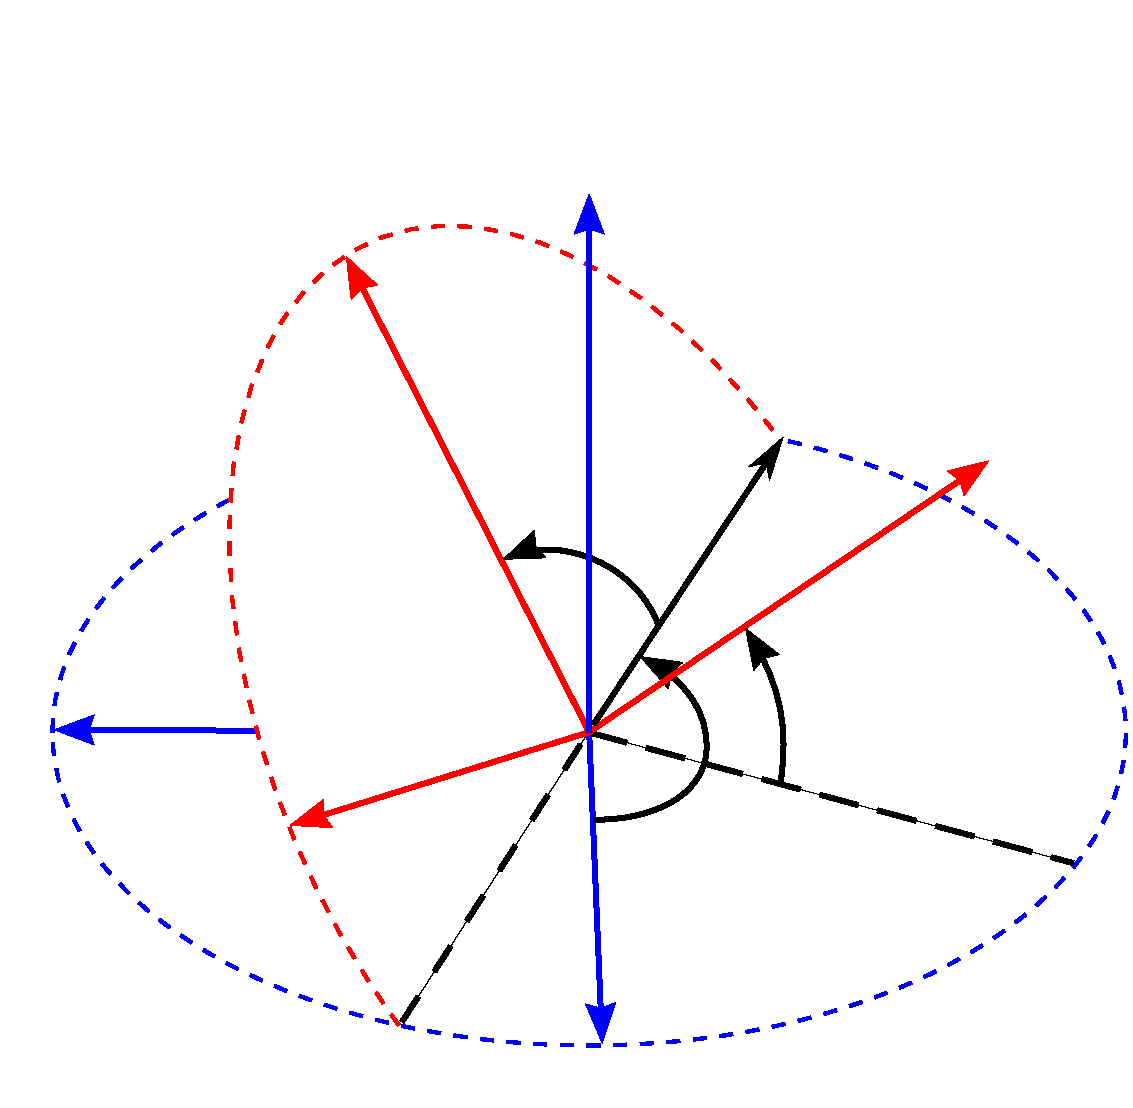
\includegraphics[width=.7\textwidth]{Figures/taitbryan.pdf}};
    
\node [] at (0.5,0.2) {$\phi$};
\node [] at (0.65,-1.85) {$\psi$};
\node [] at (1.55,-0.9) {$\theta$};

\node [] at (-3.4,-1.1) {$x$};
\node [] at (0.25,-3.3) {$y$};
\node [] at (0.12,2.43) {$z$};

\node [] at (2.8,0.6) {$X$};
\node [] at (-1.5,2.05) {$Y$};
\node [] at (-2.0,-1.7) {$Z$};
\end{tikzpicture}
\caption{Representation of the body frame (red) with respect to the world frame (blue). The body frame was rotated, by the Euler angles $\psi, \theta, \phi$ about the axes $z, y', X$, respectively, from \cite{Wiki_taitbryan}.} \label{fig:Euler_angles}
\end{figure}

Euler angles are a simple and intuitive means to represent rotations in three-dimensional space. However, for the above mentioned parameterisation they have singularities at values of $\theta = n \pi$, $n \in \mathbb{Z}$. At these points a rotation about the $x$-axis and the $z$-axis constitute the same motion, which results in the loss of one degree of freedom and makes changes in $\phi$ and $\psi$ indistinguishable. This phenomenon is called \emph{gimbal lock}.

\subsection{Transformation Matrix}

Coordinates representing a point in one coordinate system can be transformed to another. Such a transformation can be expressed as a multiplication of a matrix with the coordinate vector that is to be transformed. Let $\mathbf{E}$ denote the orthonormal basis $\{x, y, z\} \in \mathbb{R}^3$ and let $\mathbf{E}'$ denote the orthonormal basis $\{X, Y, Z\} \in \mathbb{R}^3$. Furthermore, let $\mathbf{p}$ denote the position vector of an arbitrary point in three-dimensional Euclidean space. The coordinate transformation from $\mathbf{E}$ to $\mathbf{E}'$ is denoted $\bm{\Omega}_{\mathbf{E} \rightarrow \mathbf{E}'}: (p_1, p_2, p_3) \mapsto (p'_1, p'_2, p'_3)$. Then, the linear transformation from $\mathbf{p}$ to $\mathbf{p}'$ is given by

\begin{equation}\label{eq:transformation}
  \mathbf{p'} = \bm{\Omega}_{\mathbf{E} \rightarrow \mathbf{E}'}(\mathbf{p}) = \mathbf{T} \mathbf{p}\,,
\end{equation}

\noindent
where $\mathbf{T}$ is the \emph{transformation matrix}, which is a function of the rotation angles between the two coordinate systems.

In order to transform the coordinate vector from the \emph{world frame} to the \emph{body frame}, according to the common aerospace rotation sequence mentioned above and the \gls{NED} coordinate system, the transformation matrix $\mathbf{C}_{wb}$ is given by

\begin{equation}\label{eq:transformation_matrices}
\begin{split}
\mathbf{C}_{wb} & = \mathbf{T}_x(\phi) \mathbf{T}_y(\theta) \mathbf{T}_z(\psi) \\
 & = {\left[ \begin{smallmatrix}
    1 \; & 0 \; & 0 \\
    0 \; & \cos \phi \; & \sin \phi \\
    0 \; & -\sin \phi \; & \cos \phi
    \end{smallmatrix}\right]}
    {\bigg[ \begin{smallmatrix}
    \cos \theta \; & 0 \; & -\sin \theta \\
    0 \; & 1 \; & 0 \\
    \sin \theta \; & 0 \; & \cos \theta
    \end{smallmatrix} \bigg]}
    {\left[\begin{smallmatrix}
    \cos \psi \; & \sin \psi \; & 0 \\
    -\sin \psi \; & \cos \psi \; & 0 \\
    0 \; & 0 \; & 1
    \end{smallmatrix}\right]}\\
 & = {\left[\begin{smallmatrix}
   \cos \theta \cos \psi \; &
    \cos \theta \sin \psi \; &
   -\sin \theta \\
    \sin \phi \sin \theta \cos \psi - \cos \phi \sin \psi \;\; &
    \sin \phi \sin \theta \sin \psi + \cos \phi \cos \psi \;\; &
    \sin \phi \cos \theta \\
    \cos \phi \sin \theta \cos \psi + \sin \phi \sin \psi \;\; &
    \cos \phi \sin \theta \sin \psi - \sin \phi \cos \psi \;\; &
    \cos \phi \cos \theta
  \end{smallmatrix}\right]}
\end{split}
\end{equation}

\noindent
Plugged in Equation \ref{eq:transformation} ($\mathbf{T} = \mathbf{C}_{wb}$), the pre-multiplications of the matrices $\mathbf{T}_x(\phi), \mathbf{T}_y(\theta), \mathbf{T}_z(\psi)$ to the vector $\mathbf{p}$ represent the coordinate rotations about the single axes $x, y', Z$, according to the right hand rule, respectively. That is, the function $\bm{\Omega}_{\mathbf{E} \rightarrow \mathbf{E}'}$ maps the vector $\mathbf{p}$ to its orthogonal projection onto the axes of the coordinate system, which result from the respective two-dimensional rotation of $\phi, \theta, \psi$ about the axes $x, y', Z$. This is illustrated for a single rotation around the $z$-axis by the angle $\psi$ in Figure \ref{fig:transformation_matrix}. Note that $\{x', y', z'\}$ denotes the coordinate frame after the first elemental rotation. The matrices $\mathbf{T}_x(\phi), \mathbf{T}_y(\theta)$, and $\mathbf{T}_z(\psi)$ are also known as direction cosine matrices, since their elements are the cosines of the unsigned angles between the body-fixed axes and the axes of the world frame, as shown in \cite{diebel2006attitude}. The form stated here is already simplified. The matrix $\mathbf{C}_{bw}$ that transforms a coordinate vector from the body frame to the world frame is given by

\begin{figure}[t]
\centering

\tdplotsetmaincoords{60}{110}

\begin{tikzpicture}[scale=6,tdplot_main_coords]

\coordinate (O) at (0,0,0);
\pgfmathsetmacro{\psivec}{55}
\tdplotsetcoord{P}{0.8}{44}{\psivec}

\draw[thick,->] (0,0,0) -- (.8,0,0) node[anchor=north west]{$x$};
\draw[thick,->] (0,0,0) -- (0,.8,0) node[anchor=north west]{$y$};

\tdplotsetrotatedcoords{0}{0}{25}

\draw[thick,blue,tdplot_rotated_coords,->] (0,0,0) -- (.8,0,0) node[anchor=north west]{$x'$};
\draw[thick,blue,tdplot_rotated_coords,->] (0,0,0) -- (0,.8,0) node[anchor=west]{$y'$};
\draw[very thick,blue,tdplot_rotated_coords] (0,0,0) -- (0, 0.25, 0) node[anchor=south east]{$p_y'$};
\draw[thick,blue,tdplot_rotated_coords,->] (0,0,0) -- (0,0,.8) node[anchor=north west]{$z'=z$};
\draw[very thick,blue,tdplot_rotated_coords] (0,0,0) -- (0.507, 0, 0) node[pos=0.9, label={left:$p_x'$}, rounded corners=1pt]{};
\draw[very thick,blue,tdplot_rotated_coords] (0,0,0) -- (Pz) node[pos=0.5, label={left:$p_z'$}]{};

%draw a vector from origin to point (P) 
\draw[-stealth,color=red] (O) -- node [anchor=south]{$p$}(P);

%draw projection on xy plane, and a connecting line
\draw[dashed, red] (O) -- (Pxy);
\draw[dashed, red] (P) -- (Pxy);
\draw[dashed] (Px) -- (Pxy);
\draw[dashed] (Py) -- (Pxy);

\tdplotdrawarc[-stealth]{(0,0,0)}{0.58}{0}{25}{anchor=north}{$\psi$}

\draw[dashed] (0.8,0,0) arc (0:115:0.8);

\draw[dashed, blue, tdplot_rotated_coords] (0.507, 0, 0) -- (Pxy);
\draw[dashed, blue, tdplot_rotated_coords] (0, 0.25, 0) -- (Pxy);
\draw[dashed, blue, tdplot_rotated_coords] (P) -- (Pz);

\end{tikzpicture}
\caption{An exemplary coordinate rotation about the $z$-axis by an angle $\psi$, illustrating the orthogonal projection on the resulting axes $x', y', z'$.}
	\label{fig:transformation_matrix}
\end{figure}


\begin{equation}
\mathbf{C}_{bw} = {\left[\begin{smallmatrix}
   \cos \theta \cos \psi \; &
    \sin \phi \sin \theta \cos \psi - \cos \phi \sin \psi \; &
    \cos \phi \sin \theta \cos \psi + \sin \phi \sin \psi \\
    \cos \theta \sin \psi \;\; &
    \sin \phi \sin \theta \sin \psi + \cos \phi \cos \psi \;\; &
    \cos \phi \sin \theta \sin \psi - \sin \phi \cos \psi \\
    -\sin \theta \;\; &
    \sin \phi \cos \theta \;\; &
    \cos \phi \cos \theta
  \end{smallmatrix}\right]}
\end{equation}

\noindent
Note that $\mathbf{C}_{bw} = \mathbf{C}^T_{wb} = \mathbf{C}^{-1}_{wb}$. Thus, $\mathbf{C}^{ }_{bw}$ and $\mathbf{C}_{wb}$ are orthogonal matrices so that $\mathbf{C}^{ }_{bw} \mathbf{C}_{wb} = \mathbf{I}_3$, where $\mathbf{I}_3 \in \mathbb{R}^{3 \times 3}$ is the identity matrix.

\section{Projection of the Gravity Vector}\label{sec:projection_gravity}

% and Earth's Magnetic Field Vector

As described in Section \ref{sec:accelerometers}, accelerometers measure the linear acceleration they experience. Under static or quasi-static conditions, that is, the sensor is in uniform motion, or at low acceleration, it can be assumed that the measured acceleration is mainly that of gravity. By means of simple trigonometric functions estimates for the pitch and the roll angle can be obtained. Since the gravity vector is perpendicular to the $xy$-plane, and thus a rotation around the $z$-axis will not cause any variation in the sensed acceleration, the yaw angle cannot be obtained by this method. To solve this problem a three-dimensional magnetometer is used, which measures the variation of Earth's magnetic field while rotating around the $z$-axis.

When the accelerometer is motionless, its measurements will be directly related to the angle of the sensor relative to gravity, as depicted in Figure \ref{fig:acceleration_motion} (a). In that case $\theta$ with respect to the vertical is given by

\begin{equation} \label{eq:projection_gravity}
  \theta = \mbox{atan}2(A_z, A_x)\,,
\end{equation}

\noindent
where $A_x$ and $A_z$ are the components of the acceleration vector in $x$ and $z$-direction, respectively. However, when the sensor is in motion, in addition to the gravity, there are radial and tangential acceleration components due to motion, as depicted in Figure \ref{fig:acceleration_motion} (b). The magnitude of the gravity vector $\mathbf{g}$ is denoted with $\|\mathbf{g}\|$. Ignoring these components will cause incorrect angle estimates.

\begin{figure}
\centering
\begin{subfigure}[]{0.45\textwidth}
\caption{}
\begin{tikzpicture}[auto, thick, node distance=3cm,>=latex']
    \node [draw, very thick, rounded corners=1pt, rectangle, minimum height=6em, minimum width=3em, align=center, rotate around={27:(-1,0.5)}] (sensor) {Sensor};
    \node[coordinate] (A) at (0.7, -0.6) {};
    \node[coordinate] (B) at (1.95, -3) {};
    \node[coordinate] (C) at (0.7, -3.56) {};
    
    \draw[->] (A) -- node[name=x] {$A_x = \|\mathbf{g}\| \cos \theta$}(B);
    \draw[->] (B) -- node[name=y] {$A_z = \|\mathbf{g}\| \sin \theta$}(C);
    \draw[->, very thick] (A) -- node[name=g, label={left:$\mathbf{g}$}] {}node [pos=0.35]{$\theta$} (C);
  
 	\draw[-stealth] (0.7,-2.0) arc (270:297:1.4);
      
    \end{tikzpicture}
\end{subfigure}
\quad
\begin{subfigure}[]{0.45\textwidth}
\caption{}
\begin{tikzpicture}[auto, thick, rounded corners=1pt, node distance=3cm,>=latex']
    \node [draw, very thick, rectangle, minimum height=6em, minimum width=3em, align=center, rotate around={27:(-1,0.5)}] (sensor) {Sensor};
    \node[coordinate] (A) at (0.7, -0.6) {};
    \node[coordinate] (B) at (2.1, -3.55) {};
    \node[coordinate] (C) at (0.7, -3.56) {};
    \node[coordinate] (D) at (1.2, -4) {};
    
    \draw[->, red, very thick] (A) -- node[name=d] {} (D);
    \draw[->] (A) -- node[name=x] {$A_x = A_{rad} + \|\mathbf{g}\| \cos \theta$} node [pos=0.46, label={left:$\theta$}]{} (B);
    \draw[->] (B) -- node[name=y] {$A_z = A_{tan} + \|\mathbf{g}\| \sin \theta$} (D);
    \draw[->, very thick] (A) -- node[name=g, label={left:$\mathbf{g}$}] {}(C);
      
    \draw[-stealth] (0.953,-2.2) arc (270:304:0.8);  
      
    \end{tikzpicture}	
\end{subfigure}

\caption{Acceleration seen by the sensor (b) with and (a) without motion, from \cite{bennett_motion_2014}.} \label{fig:acceleration_motion}
\end{figure} 

\section{Integration of the Angular Rate}\label{sec:integration_angular}

Another way to estimate the attitude of an object is the integration of the angular rate around the $x, y$ and $z$-axis, respectively. Although this would theoretically lead to very accurate orientation estimates, they are impaired by \gls{ARW} and dynamical bias in practice. \gls{ARW} is an effect caused by the integration of high-frequency, thermo-mechanical noise, which leads to a random additive angle in the orientation signal. An even greater impact than AWR has the gyroscope's dynamic bias, which has its origin in low-frequency flicker noise. Both effects cause a dramatical drift in the angle signal over time.

\section{Sensor Fusion}

Since the projection of the gravity vector is only valid under static or quasi-static conditions, or at low acceleration, and the integration of the angular rate leads to non-reliable estimates due to \gls{ARW} and dynamic bias, but is not affected by the intensity of motion, a means to combine the information of both sensors is desirable. The combination of information from multiple sensors to increase the overall precision of the estimation of a certain quantity of interest is termed \emph{sensor fusion}. \citeauthor{raol2009multi} \cite{raol2009multi} states the following advantages of sensor fusion:
 
\begin{itemize}
\item Robust functional and operational performance is given, in case of data loss from one sensor, due to redundancy provided by multiple sensors.
\item Enhanced confidence in the results inferred from the measurement of one sensor, if they are confirmed by the measurement of another sensor.
\item With sensor fusion an arbitrary fine time resolution of measurements is possible, whereas single sensors need a finite time to transmit measurements and so limit the frequency of measurements.
\item One sensor might be, to some extent, better in a certain state of the measured process, e.\,g. low or high motion intensity in attitude estimation, and thus, by fusing multiple sensor signals, a satisfactory accuracy among all states of the process could be attained.
\end{itemize}

\noindent
Sensor fusion can be realised by the use of a Kalman filter. This specific digital filter is described in detail in the next chapter, and applied in Chapter \ref{ch:Implementation} to fuse the sensor signals of accelerometers and gyroscopes.


